% MLP 2 hidden layers


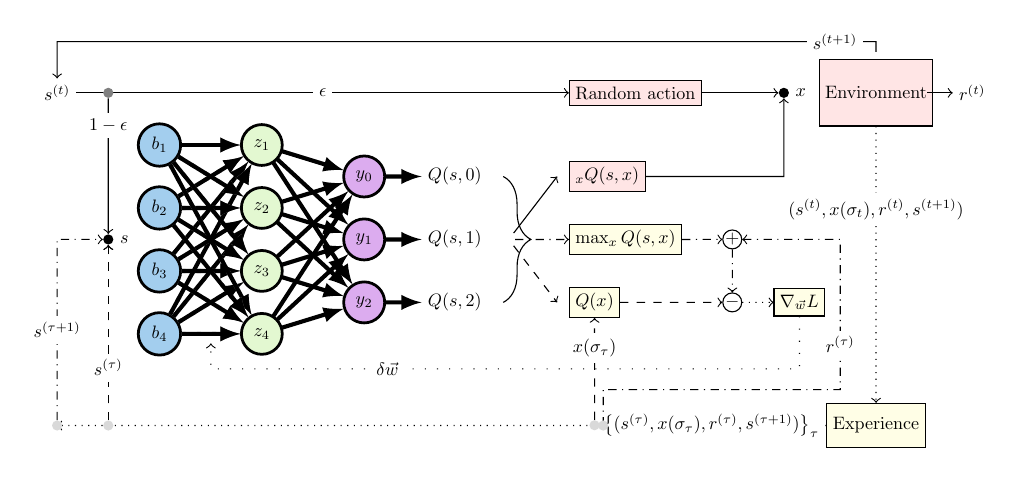
\begin{tikzpicture}[scale=.65,every node/.style={scale=0.65}]
    \usetikzlibrary{shapes,arrows,positioning,calc,chains,scopes}

% colors
\definecolor{snowymint}{HTML}{E3F8D1} % light green -yellow
\definecolor{wepeep}{HTML}{FAD2D2} % pink
\definecolor{portafino}{HTML}{F5EE9D} % light yellow
\definecolor{plum}{HTML}{DCACEF} % purple
\definecolor{sail}{HTML}{A3CEEE} % light blue
\definecolor{highland}{HTML}{6D885A} % dark green

\tikzstyle{signal}=[arrows={-latex},draw=black,line width=1.5pt,rounded corners=4pt]

% RNN
\tikzstyle{block}=[draw=black,line width=1.0pt]
\tikzstyle{cell}=[style=block,draw=highland,fill=snowymint,
    rounded corners]
\tikzstyle{celllayer}=[style=block,draw,fill=portafino,
    inner sep=1pt,outer sep=0,
    minimum width=28pt, minimum height=14pt]
\tikzstyle{pointwise}=[style=block,ellipse,fill=wepeep,
    inner sep=1pt,outer sep=0, minimum size=12pt]

\def\iolen{24pt}
\def\intergape{2pt}

% MLP and CNN
\tikzstyle{netnode}=[circle, inner sep=0pt, text width=22pt, align=center, line width=1.0pt]
\tikzstyle{inputnode}=[netnode, fill=sail,draw=black]
\tikzstyle{hiddennode}=[netnode, fill=snowymint,draw=black]
\tikzstyle{outputnode}=[netnode, fill=plum,draw=black]

% Architecture
\def\layerwidth{90pt}
\def\layerheight{14pt}

\tikzstyle{layer}=[style=block, draw, fill=black!20!white,
    inner sep=1pt,outer sep=0, font=\footnotesize,
    text centered, 
    minimum width=\layerwidth, minimum height=\layerheight]

\tikzstyle{fc}=[style=layer, fill=blue!30!white]
\tikzstyle{conv}=[style=layer, fill=green!30!white]
\tikzstyle{activation}=[style=layer, fill=orange!30!white]
\tikzstyle{pool}=[style=layer, fill=red!30!white]
\tikzstyle{bn}=[style=layer, fill=cyan!30!white]
\tikzstyle{recurrent}=[style=layer, fill=purple!30!white]
\tikzstyle{softmax}=[style=layer, fill=yellow!30!white]
\tikzstyle{point}=[]
\tikzstyle{branch}=[coordinate]

\def\vlayerwidth{30pt}
\def\vlayerheight{3pt}
\def\vblockheight{28pt}

\tikzstyle{vlayer}=[minimum width=\vlayerwidth, minimum height=\vlayerheight]
\tikzstyle{vblock}=[minimum width=\vlayerwidth, minimum height=\vblockheight, text width=1cm, align=center]


% Precision, Recall
\colorlet{fn}{gray!90!green!30!white}
\colorlet{tp}{green!40!white}
\colorlet{fp}{red!40!white}
\colorlet{tn}{gray!90!red!20!white}
    
    
    
    \def\nodedist{35pt}
    \def\layerdist{2}
    \def\pindist{20pt}
    
    \tikzstyle{every pin edge}=[signal]
    \tikzstyle{annot} = [text width=4em, text centered]
    
    % define blocks top left corners
    %% state block %%
    \def\statex{4}
    \def\statey{0}
    %% epsilon block %%
    \def\epsilonx{4}
    \def\epsilony{2}
    %% 1-epsilon block %%
    \def\epsilonx{4}
    \def\epsilony{6}
    %% NN block %%
    \def\nnx{6}
    \def\nny{6}
    %% argmax block %%
    \def\argmaxx{14}
    \def\argmaxy{{\nny-0.5*\nodedist-\nodedist}}
    %% random block %%
    \def\randomx{\argmaxx}
    \def\randomy{\statey}
    %% max Q(a) block %%
    \def\maxqax{14}
    \def\maxqay{{\nny-0.5*\nodedist-2*\nodedist}}
    %% Q(a) block %%
    \def\qax{14}
    \def\qay{{\nny-0.5*\nodedist-3*\nodedist}}
    %% loss block %%
    \def\lossx{18}
    \def\lossy{\qay}
    %% ENV block %%
    \def\envx{20}
    \def\envy{0}
    %% experience block %%
    \def\experiencex{\envx}
    \def\experiencey{-6.5}
    %% adder block %%
    \def\addx{{\maxqax+3}}
    \def\addy{\maxqay}
    %% minus block %%
    \def\minusx{{\addx}}
    \def\minusy{\qay}
    
    %%%%%%%%%%%%%%%%%
    %% State block %%
    %%%%%%%%%%%%%%%%%
    \def\xx{\statex}
    \def\yy{\statey}
    \node (state) [] at (\xx, \yy) { $s^{(t)}$};
    
    
    %%%%%%%%%%%%%%%%%
    %% random block %%
    %%%%%%%%%%%%%%%%%
    \def\xx{\randomx}
    \def\yy{\randomy}
    \node (random) [rectangle,draw,anchor=west,fill=red!10] at (\xx,\yy) {Random action};
    
    %%%%%%%%%%%%%%%%%
    %% loss block %%
    %%%%%%%%%%%%%%%%%
    \def\xx{\lossx}
    \def\yy{\lossy}
    \node (loss) [rectangle,draw,anchor=west,fill=yellow!10] at (\xx,\yy) {$\nabla_{\vec{w}} L$};    
    
    %%%%%%%%%%%%%%%%%
    %% argmax block %%
    %%%%%%%%%%%%%%%%%
    \def\xx{\argmaxx}
    \def\yy{\argmaxy}
    \node (argmaxQ) [rectangle,draw,anchor=west,fill=red!10] at (\xx,\yy) {$\argmax_x Q(s,x)$};
    
    %%%%%%%%%%%%%%%%%
    %% max Q(a) block %%
    %%%%%%%%%%%%%%%%%
    \def\xx{\maxqax}
    \def\yy{\maxqay}
    \node (maxQ) [rectangle,draw,anchor=west,fill=yellow!10] at (\xx,\yy) {$\max_x Q(s,x)$};
    
    %%%%%%%%%%%%%%%%%
    %% Q(a) block %%%
    %%%%%%%%%%%%%%%%%
    \def\xx{\qax}
    \def\yy{\qay}
    \node (Qa) [rectangle,draw,anchor=west,fill=yellow!10] at (\xx,\yy) {$Q(x)$};
    
    %%%%%%%%%%%%%%%%%
    %% adder block %%%
    %%%%%%%%%%%%%%%%%
    \def\xx{\addx}
    \def\yy{\addy}
    \node (adder) [circle,inner sep=0.1,draw,anchor=west] at (\xx,\yy) {$+$};
    
    %%%%%%%%%%%%%%%%%
    %% minus block %%%
    %%%%%%%%%%%%%%%%%
    \def\xx{\minusx}
    \def\yy{\minusy}
    \node (minus) [circle,inner sep=0.1,draw,anchor=west] at (\xx,\yy) {$-$};
    
    
    %%%%%%%%%%%%%%%%%
    %% ENV block %%
    %%%%%%%%%%%%%%%%%
    \def\xx{\envx}
    \def\yy{\envy}
    \node (env) [rectangle,inner ysep=15pt,draw,anchor=center,fill=red!10] at (\xx,\yy) {Environment};
    \node (actiondot) [circle,fill=black,inner sep=2pt,label=right:$x$] at (\xx-1.8,\yy) {};
    
    
    %%%%%%%%%%%%%%%%%
    %% experience block %%
    %%%%%%%%%%%%%%%%%
    \def\xx{\experiencex}
    \def\yy{\experiencey}
    \node (experience) [rectangle,inner ysep=8pt,draw,anchor=center,fill=yellow!10] at (\xx,\yy) {Experience};
    
    
    %%%%%%%%%%%%%%
    %% NN BLOCK %%
    %%%%%%%%%%%%%%
    % set reference point to the NN block
    \def\xx{\nnx}
    \def\yy{\nny}
    
    \node (indot) [circle,fill=black,inner sep=2pt,label=right:$s$] at (\xx-1,\yy-2.5*\nodedist) {};

    % Input layer neurons
    \foreach \y in {1,...,4}
        \node[inputnode] 
            (I\y) at (\xx,\yy-\y*\nodedist) {$b_{\y}$};  

    % Hidden layer neurons
    \foreach \y in {1,...,4}
        \node[hiddennode] 
            (H\y) at 
            (\xx+\layerdist,\yy-\y*\nodedist) {$z_{\y}$};
            %($(\xx+\layerdist,\yy-\y*\nodedist) +(0, 0.5*\nodedist)$) {$z_{\y}$};
    
    % Output layer
    \foreach \y in {0,...,2}
        \node[outputnode, pin={[pin edge={-latex}, pin distance=\pindist]right:$Q(s,\y)$}]
            (O\y) at (\xx+2*\layerdist, {\yy-0.5*\nodedist-(\y+1)*\nodedist}) {$y_{\y}$};

    \foreach \dest in {1,...,4}
        \foreach \source in {1,...,4}
            \ifthenelse{\source=4}{\draw[signal, loosely dotted,color=gray] (I\source) -- (H\dest);}{\draw[signal] (I\source) -- (H\dest);};

    
    \foreach \dest in {0,...,2}
        \foreach \source in {1,...,4}
            \draw[signal] (H\source) edge (O\dest);
            
    % Brace
        \draw [decorate,decoration={brace,amplitude=10pt,raise=4pt},xshift=0pt] ($(O0)+(2.5,0)$) -- ($(O2)+(2.5,0)$) node (braceOut) [black,midway,right, xshift=0.2cm] {};
            
    %\node[annot, above=4pt of H11] (hl) {Hidden layer 1};
    %\node[annot] at (I1 |- hl) {Input layer};
    %\node[annot] at (O1 |- hl) {Output layer};
    %%%%%%%%%%%%%%%%%%
    %% end NN BLOCK %%
    %%%%%%%%%%%%%%%%%%
    
    
    %%%%%%%%%%%%%%%%%%%%
    %% TRAINING FLOWS %%
    %%%%%%%%%%%%%%%%%%%%
    \coordinate[left = 0.15cm of argmaxQ] (argmaxQL);
    \coordinate[left = 0.15cm of Qa] (QaL);
    \draw[->] (braceOut) -- (argmaxQL) ;
    \draw[dashdotted,->] (braceOut) -- (maxQ) ;
    \draw[dashdotted,->] (maxQ) -- (adder);
    \draw[dashed,->] (braceOut) -- (QaL) ;
    \draw[dashed,->] (Qa) -- (minus);
    \draw[dashdotted,->] (adder) -- (minus);
    \draw[dotted,->] (minus) -- (loss);
    \draw[loosely dotted,->] (loss) -- ($(loss) - (0,1.3)$) -- node[pos=0.7,fill=white] {$\delta\vec{w}$} ($(loss)-(0,1.3)-(11.5,0)$) -- ($(loss)-(0,0.8)-(11.5,0)$);
    % experience replay BUS
    \draw[dotted,->] (experience) -- node (sarsa) [pos=0.15,fill=white] {$\left\{ (s^{(\tau)}, x(\sigma_\tau), r^{(\tau)}, s^{(\tau+1)})\right\}_\tau$} ($(\nnx,\experiencey)-(2,0)$)  node (stau)[circle,fill=gray!30,inner sep=2] at ({\xx-1,\experiencey}) {} node (stau1)[circle,fill=gray!30,pos=1,inner sep=2]{} node (atau) [circle,fill=gray!30,inner sep=2] at ($(Qa) - (0,2.4)$){};
    \draw[dashdotted,->] let \p1 = (sarsa), \p2 = (loss), \p3 = (adder) in (\x1-60,\y1) -- node[circle,fill=gray!30,pos=0,inner sep=2]{} (\x1-60,\y1+20) -- (\x3+60,\y1+20) -- node[pos=0.3,fill=white] {$r^{(\tau)}$} (\x3+60,\y3) -- (adder);
    % experience replay input
    \draw[dashed,->] (atau) -- (Qa) node [pos=0.7,fill=white] {$x(\sigma_\tau)$};
    \draw[dashed,->] (stau) -- (indot) node [pos=0.3,fill=white] {$s^{(\tau)}$};
    \draw[dashed,->] (stau) -- (indot) node [pos=0.3,fill=white] {$s^{(\tau)}$};
    \draw[dashdotted,->] let \p1 = (indot),\p2 = (stau1) in (stau1) -- node [pos=0.5,fill=white] {$s^{(\tau+1)}$} (\x2,\y1) -- (indot);
    
    %%%%%%%%%%%%%%%%%%%%%
    %% EXECUTION FLOWS %%
    %%%%%%%%%%%%%%%%%%%%%
    \draw[->,fill=black] let \p1 = (indot) in (state) -- (random) node (epsilon) [circle,fill=gray,inner sep=2] at (\x1,\statey) {} node [pos=0.5,fill=white] {$\epsilon$};
    \draw[->] (epsilon) -- node [pos=0.2,fill=white] {$1-\epsilon$} (indot);
    \draw[->] (random) -- (actiondot); 
    \draw[->] let \p1 = (actiondot), \p2 = (argmaxQ) in (argmaxQ) -- (\x1,\y2) -- (actiondot); 
    \draw[->]  (\envx,\envy+0.8) -- (\envx,{\envy+1}) -- node [pos=0.05,fill=white] {$s^{(t+1)}$} (\statex,\statey+1) -- (state); 
    \draw[->] (\envx+1,\envy) -- (\envx+1.5,\envy) node [right] {$r^{(t)}$};
    \draw[dotted,->] (env) -- node [pos=0.3,fill=white] {$(s^{(t)}, x(\sigma_t), r^{(t)}, s^{(t+1)})$} (experience);
    

\end{tikzpicture}
